% Para documento texto corto
\documentclass[paper=a4,oneside,fontsize=12pt]{scrartcl}
%\documentclass[paper=letter,oneside,fontsize=12pt, 
% parskip=full]{scrartcl}

% Establecer dimensiones de los margenes
%\ usepackage[inner=1.5cm,outer=3cm,top=2cm,bottom=4cm,
%	bindingoffset=5mm]{geometry}
\usepackage[left=3cm,right=3cm,top=3cm,bottom=3cm,
bindingoffset=0cm]{geometry}

% Permite ingresar caracteres acentuados y especiales 
% sin necesidad de emplear comando
% utf8 codificacion de entrada Unicode (mas simbolos que ASCII)
\usepackage[utf8]{inputenc}

% T1 encoding for European, English, American text
\usepackage[T1]{fontenc}
% Fuente escalable
\usepackage{lmodern}

% Carga babel, idioma ingles
\usepackage[english,spanish]{babel}

% Mejor jsutificacion, tipografia alta calidad.
\usepackage{microtype}

% Agrega comandos extra al comando tabular
% \toprule, \midrule, \bottomrule
\usepackage{booktabs}
% Tablas con ancho establecido por usuario
\usepackage{tabularx}
% Para posicionamiento preciso de tablas dentro del texto
\usepackage{float}

% Encabezados personalizados
\usepackage{fancyhdr}
\usepackage{graphicx}

% Permite obtener el numero de la ultima pagina
\usepackage{lastpage}

% Paquetes para figuras
% Paquete caption para titulos figuras
% Paquete subcaption para subfiguras
\usepackage{caption}
\usepackage{subcaption}

% Cabeceras
\pagestyle{fancy}
% Borra cabecera y pie actuales
\fancyhead{}
% Cintillo cabecera
%\chead{
%	
\includegraphics[width=150mm]{Imagenes/Cabecera.png}
%}
\fancyhead[L]{
\includegraphics[width=150mm]{Imagenes/Cabecera.png}}
\fancyfoot[C]{
	\begin{tabular}{|m{2.0cm}|m{10.0cm}|m{2.0cm}|}
		\hline
		\centering Versión 0.1	& 
		\centering 
\includegraphics[height=0.8cm]{Imagenes/Pie.png} & 
		{\centering  \thepage / \pageref{LastPage}} \\			
		\hline 
	\end{tabular}}

% Numeracion de paginas
% numeros arabigos
\pagenumbering{arabic}

% Comando que define el nombre la aplicacion
\newcommand{\AppName}{\textsc{CenditLab}\ }

% Comando que define el nombre del sistema de medición de figura de ruido
\newcommand{\smr}{sistema de medición de ruido}
\newcommand{\SMR}{SMR}

% Comando que define el nombre del Cendit
\newcommand{\cendit}{Cendit}

\begin{document}
	
	\begin{titlepage}
				
		\begin{center}	
			
			\vspace{10cm}
			
			\begin{Large}			
				Especificación de Requisitos de Software
			\end{Large}
		
			\begin{Huge}
				\textsc{\AppName}
			\end{Huge}
			
		\end{center}
		
	\end{titlepage}

	\tableofcontents
	
	\section{Introducción}
	Esta sección brinda un panorama general del contenido del presente documento de especificaciones de requisitos de software. Se da al final una lista de abreviaturas.
	
	\subsection{Propósito}
	El propósito de este documento es dar una descripción detallada de los requerimientos para el software \AppName. Ilustrará el propósito y sentará de manera formal y completa la base inicial para el proceso de desarrollo. Explicará la restricciones del sistema, interfaces e interacciones con aplicaciones externas. 
	
	Este documento se dirige principalmente a los futuros usuarios de la software \AppName para fines de aprobación, y para desarrolladores, que se involucren en un futuro en el soporte y mejoras de la base de código.
	
	\subsection{Alcance}
	
	El software \AppName es una aplicación de escritorio que brinda a los usuarios del \emph{\smr} un entorno de trabajo o laboratorio virtual 
	
	El software \AppName es una aplicación para PC de escritorio que sirve como interfaz de software para el \emph{\smr} presente en el \cendit. Permite realizar muchas de las tareas propias de los equipos de un \smr dentro de un entorno de trabajo en una aplicación centralizada, o laboratorio virtual. 
	
	\AppName permite a los usuarios realizar mediciones de manera automatizada y remota, configuración los instrumentos instrumentos del \smr, capturar y visualizar de datos además de generar reportes en formatos digitales, como pdf o html.
	
	\AppName utiliza la capacidad de transferencia de datos a través de buses de comunicaciones que disponen los instrumentos del \smr, como GPIB, USB o LAN. Para ello el PC donde se ejecute la aplicación debe disponer de los aditamentos de hardware apropiado que permitan acceder a estos buses, asi como también el respectivo soporte de software en forma de librerías o controladores de dispositivo, que permitan a un PC el acceso a estos buses.
	
	\subsection{Definiciones, acronimos y abreviaturas}
	
	\begin{table}[h!]
		\begin{tabular}{|p{4cm}|p{10cm}|} 
			\hline
			Termino & Definición \\
			\hline
		\end{tabular}	
	\end{table}

	\subsection{Referencias}
	% 	\bibliographystyle{acm}	
	% 	\bibliographystyle{abbrv}	
	% 	\bibliographystyle{apalike}
	
	%\bibliographystyle{ieeetr}
	%\bibliography{Bibliografia}
	
	\begingroup
		\renewcommand{\section}[2]{}
		\begin{thebibliography}{9}
			\bibitem{iso-29148} 
			ISO/IEC/IEEE 29148. 
			\textit{Systems and software engineering - Lyfe cycle processes - Requirements enginering}. 
			ISO/IEC/IEEE, 2011.
			
			\bibitem{iso-42010} 
			ISO/IEC/IEEE 42010. 
			\textit{Systems and software engineering - Architecture description}. 
			ISO/IEC/IEEE, 2011.		
			
			\bibitem{softwareengineering-narang} 
			Rajesh Narang. 
			\textit{Software Engineering Principles and Practices}. 
			Mc Graw Hill, New Delhi, India, 2015.			
			
			\bibitem{softwareengineering-sommerville} 
			Ian Sommerville. 
			\textit{Software Engineering}. 
			Addison-Wesley, Boston, Massachusetts, 2011.					
			
			\bibitem{latexcompanion} 
			Michel Goossens, Frank Mittelbach, and Alexander Samarin. 
			\textit{The \LaTeX\ Companion}. 
			Addison-Wesley, Boston, Massachusetts, 2011.		
			
			\bibitem{einstein} 
			Albert Einstein. 
			\textit{Zur Elektrodynamik bewegter K{\"o}rper}. (German) 
			[\textit{On the electrodynamics of moving bodies}]. 
			Annalen der Physik, 322(10):891–921, 1905.
			
			\bibitem{knuthwebsite} 
			Knuth: Computers and Typesetting,
			\\\texttt{http://www-cs-faculty.stanford.edu/\~{}uno/abcde.html}
		\end{thebibliography}
	\endgroup

	
	\subsection{Visión general}
	
	El resto de este documento incluye tres capítulos y un apéndice. El segundo provee un panorama de la funcionalidad del sistema y su interacción con el \smr. Este capitulo además introduce los diferentes tipos de \emph{participantes} y su interacción con el sistema. Más adelante, el capitulo menciona las restricciones del sistema y las suposiciones de la aplicación.
	
	El tercer capitulo describe la especificación de requerimientos al detalle y describe las diferentes interfaces del sistema. Se emplean diferentes técnicas de especificación con el objeto de mostrar los requerimientos de manera precisa para distintas audiencias.
	
	El cuarto capitulo trata con el establecimiento de la prioridad de los requerimientos. Este incluye una motivación. Expone los motivos para los métodos de prioridad escogidos y el por que de las alternativas rechazadas.  
	
	El apéndice al final de este documento incluye los resultados de la priorización de requerimientos y el plan de entrega basado en las prioridades.
	
	\section{Descripción general}
	
	Esta sección brindará una perspectiva general de todo el sistema de software, \AppName. El sistema será explicado dentro de su contexto para mostrar como éste interactúa con el \smr por medio de su funcionalidad básica. Describirá además que tipo de participantes \textendash \emph{stakeholders} \textendash usarán el sistema y que funcionalidad estará disponible para cada tipo de ellos. Al final, se presentan las restricciones y suposiciones para el sistema.
	
	\subsection{Perspectiva de producto}
	
	\AppName será un aplicación de escritorio que servirá como interfaz de usuario de software para el \smr. El software del sistema consiste de tres partes: el soporte para interfaz gráfica, la capa de abstracción de comunicaciones y la automatizador de mediciones.
	
	\AppName será una aplicación dirigida inicialmente a PC que ejecute un sistema operativo propietario (Windows) o alguna distribución en software libre (Linux). Esto garantiza que \AppName será una aplicación portable, podrá ser ejecutada por cualquier equipo o dispositivo que posea una \emph{maquina virtual} apropiada, como JVM en Java o el entorno .NET de Microsoft, tecnologías que se encuentran disponibles bajo licencias de software libre.
	
	La aplicación resultará en una interfaz de software para los tres equipos principales que componen el \smr. En si resultará en un \emph{instrumento virtual} que concentra toda la funcionalidad del \SMR en un solo sitio: el dispositivo o PC que ejecute la aplicación.
	
	Conceptualmente se ha dividido la aplicación en cuatro grandes paquetes, como ilustra el diagrama UML de la figura \ref{Fig:DiagramaPaquetesprincipalUml}
	
	\begin{figure}[!h]
		\centering
		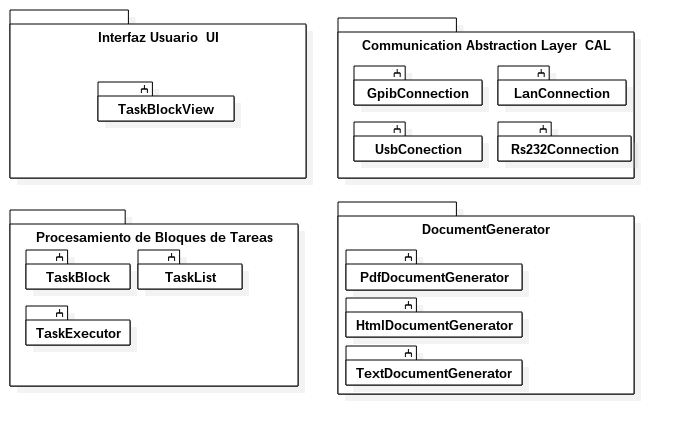
\includegraphics[width=10cm]{Imagenes/DiagramaPaquetesPrincipalUml.png}
		\label{Fig:DiagramaPaquetesprincipalUml}
		\caption{Diagrama de paquetes UML que describe la organización del software}
	\end{figure}

	La aplicación necesita establecer comunicación de datos con los instrumentos, por medio de los buses GPIB o USB, red LAN o un puerto de comunicaciones RS232. La capa en la figura \ref{Fig:DiagramaPaquetesprincipalUml} conocida como \emph{Capa de Abstracción de Comunicaciones} es la encargada de gestionar todo lo relativo a la comunicación de datos a través de múltiples interfaces o buses disponibles, mientras brinda una interfaz uniforme a las capas de software superiores.
	
	La funcionalidad de los instrumentos que componen el \SMR sera representada en software por unidades funcionales que se llamarán  \emph{bloques de tareas}. El usuario, por medio de la interfaz gráfica, podrá configurar la instrumentación agregando, conectando y programando bloques de tareas. Es responsabilidad del paquete \emph{Procesamiento de Bloques de Tareas} la compilación y ejecución de la programación hecha por el usuario.
	
	Los instrumentos presentes en el \SMR serán representados en la interfaz gráfica de la aplicación mediante diagrama de bloques. Es responsabilidad del paquete \emph{Interfaz de Usuario} la gestión de la presentación de diagramas de bloques.
	
	La aplicación \AppName presentará los resultados de una tarea de medición en pantalla o en documentos digitales en formato de documento portable (pdf), en lenguaje de marcado de hipertexto (html) o en formato de texto plano, como valores separados por comas (csv). El paquete \emph{DocumentGenerator} se encargará de cubrir esta funcionalidad.
	
	\subsection{Funciones de producto}
	
	Las tareas de medición que realizaría un usuario por medio de las interfaces físicas empleando de los instrumentos que conforman \SMR 
	podrán realizarse a través \AppName, la cual brindará una única interfaz de software al \SMR. 
	
	A través de \AppName no se necesita presencia física del usuario en el \SMR, la aplicación brindará acceso remoto a través de buses de comunicación de datos o por red LAN. 
	
	La aplicación se encargará de buscar y presentar al usuario los instrumentos que forman \SMR que se encuentren en linea, es decir, conectados a un bus de datos o a una red LAN, a la cual la PC donde se ejecute la aplicación tenga la facilidad de acceso.
	
	La funcionalidad principal de \AppName será la de automatizar el proceso de medición con el  \SMR. 
	
	La interfaz gráfica de la aplicación permitirá al usuario seleccionar los instrumentos en linea y así configurar la instrumentación adecuada para la tarea de medición, por medio de la representación gráfica de los instrumentos en forma de diagrama de bloques. Estos bloques admiten programación en forma de comandos SCPI,  estándar para instrumentos programables.
	
	El usuario podrá ejecutar la secuencia de comandos y observar los resultados en tiempo real en pantalla. La aplicación podrá además guardar los resultados de la mediciones en formatos de documento digital como pdf, html o texto plano.		
	
	\subsection{Características de los usuarios}
	
	La aplicación \AppName está dirigida a usuarios con formación técnica en el tarea de radio frecuencia, comunicaciones, antenas, electrónica y afines. En estos campos se  consideran ingenieros y técnicos universitarios como \emph{usuarios técnicos} en este documento.
	
	\subsection{Restricciones}	
	
	La aplicación \AppName requiere que en el PC o dispositivo donde se ejecute se encuentre instalada la \emph{maquina virtual} adecuada y con la versión correcta (Java Virtual Machine, JVM para Java o el entorno .NET ). 
	
	\AppName hace uso intensivo de las comunicaciones a través de los buses GPIB, USB o través de una red LAN. Por ello en el dispositivo o PC donde se ejecuta la aplicación se requiere de los periféricos de hardware apropiados, como adaptadores USB a GPIB o puente LAN a GPIB. En software también se necesita el soporte apropiado para las comunicaciones de datos, requiere de las librerías VISA de National Instruments, Linux-GPIB, VXI-11 y libUSB.	

	\subsection{Suposiciones y dependencias}	
	
	Se parte del supuesto de que el dispositivo donde se ejecute la aplicación posee la cantidad de memoria adecuada y la capacidad de procesamiento necesario para que la maquina virtual ejecute la aplicación, sin una degradación del desempeño apreciable.
	
	\section{Requerimientos específicos}
	
	Esta sección presenta todos los requerimientos funcionales y de calidad para la aplicación \AppName. Muestra un descripción detallada del sistema y de todas sus características.
	
	\subsection{Requerimientos de interfaces de usuario}
	
	\subsubsection{Interfaces de usuario}
	
	Cuando el usuario inicia la aplicación, se mostrará la pantalla inicial de la figura \ref{Fig:MainWndowUI}. Esta ventana principal de la aplicación, representa el centro de control de la aplicación ya que concentra multiples funciones en forma de controles de ventana, comúnmente llamados \emph{widgets}, que el usuario debe seleccionar para ejecutar la acción asociada este control. 
	
	En la pantalla un control en la ventana principal de la aplicación, sera llevado a otra ventana con la funcionalidad asociada al control. Por ejemplo, al seleccionar el control \emph{Buscar Instrumentos} se le presentará la ventana de \emph{Explorador de Instrumentos}. 
	
	Al seleccionar \emph{Crear tarea} el usuario sera llevado a la ventana de programación de tareas de la figura \ref{Fig:ProgramWindowUI}. Por medio del control \emph{Abrir tarea} el usuario puede cargar una tarea de medición, previamente almacenada, a la ventana de programación. Presionando el control \emph{Configurar aplicación} se presentará la ventana en donde el usuario puede ajustar la configuración global de la aplicación. Presionando el control \emph{Obtener ayuda} se presentará una ventana en donde el usuario podrá indagar por ayuda.	
	
	
	\begin{figure}[h!]
		\centering 
		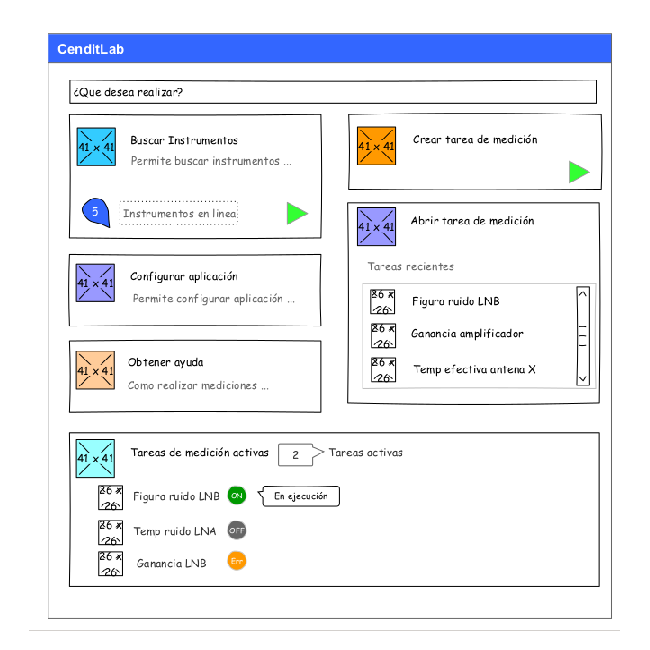
\includegraphics[width=12cm]{Imagenes/MainWindowUI.pdf}
		\label{Fig:MainWndowUI} 
		\caption{Sketch para la ventana principal de la aplicación}
	\end{figure}

	

	\begin{figure}[h!]
		\centering 
		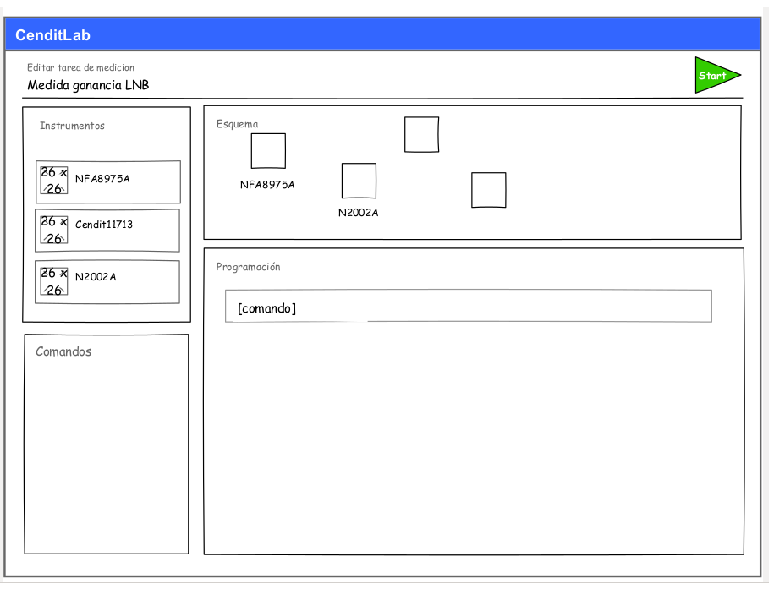
\includegraphics[width=12cm]{Imagenes/ProgramWindowUI.pdf}
		\label{Fig:ProgramWindowUI} 
		\caption{Sketch para la ventana de programación de tareas}
	\end{figure}

	\begin{figure}[h!]
		\centering 
		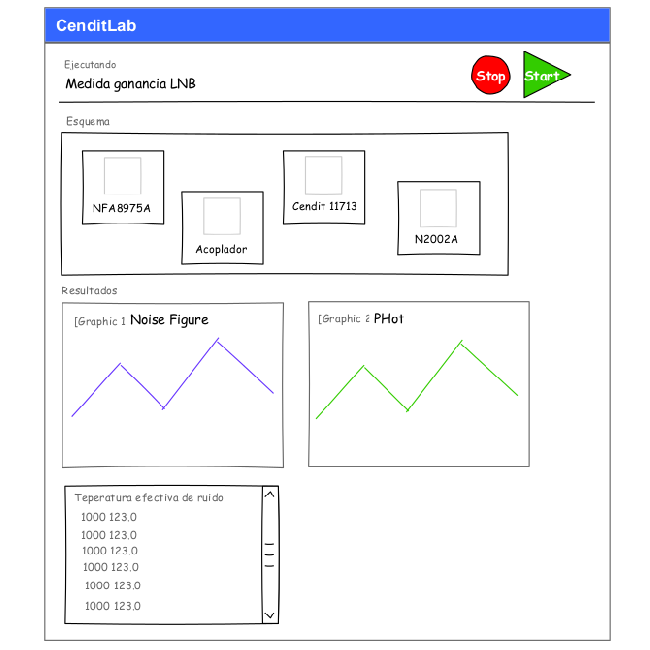
\includegraphics[width=\textwidth]{Imagenes/ExecutionWindowUI.pdf}
		\label{Fig:ExecutionWindowUi} 
		\caption{Sketch para la ventana de ejecución de tareas}
	\end{figure}
	
	\subsubsection{Interfaces de hardware}
	
	\subsubsection{Interfaces de software}
	
	\subsubsection{Interfaces de comunicaciones}
	
		% -----------------------------------------------------
		% Comando para generar formato con requisitos funcionales
		\newcommand{\funcreq}[7]{
			\subsubsection{Requerimiento funcional {#1}}

			\begin{table}[H]			
			%\begin{table}[!htbp]
				\begin{tabularx}{\textwidth}{rX}			
					\textbf{ID:} 	&	{#2}		\\
					Titulo:			&  	{#3}. 		\\
					Descripción:	&	{#4}.		\\
					Justificación: 	&	{#5}.		\\
					Dependencias:	& 	{#6}.		\\
					Usuario:		&	{#7}.		\\
				\end{tabularx}				
			\end{table}
		}
		% -----------------------------------------------------		
		
		% -----------------------------------------------------
		% Comando para generar formato con requisitos de desempeño
		\newcommand{\perfreq}[6]{
			\subsubsection{{Requerimiento de desempeño #1}}
			
			\begin{table}[H]%[!htbp]
				\begin{tabular}{rl}			
					\textbf{ID:} 	&	{#2}		\\
					Titulo:			&  	{#3}. 		\\
					Descripción:	&	{#4}.		\\
					Justificación: 	&	{#5}.		\\
					Dependencias:	& 	{#6}.		\\
				\end{tabular}				
			\end{table}
		}
		% -----------------------------------------------------				
	
	\subsection{Requerimientos funcionales}	
	
	A continuación los requerimientos funcionales
		
	\funcreq{1}
		{FR1}
			{Programar tareas de medición}
			{Los usuarios pueden programar los instrumentos y generar tareas de medición para sus posterior ejecución, de forma automatizada y remota}
			{Programar y automatizar las mediciones}
			{Ninguna}
			{Técnico}
	\funcreq{2}
		{FR2}
			{Explorador de instrumentos conectados a los buses}
			{El usuario podrá visualizar los instrumentos conectados a los buses, al cual el PC tiene acceso}
			{Con el fin de mostrar un listado de instrumentos en línea}
			{Ninguna}
			{Técnico}
	\funcreq{3}
		{FR3}
			{Configurar los instrumentos de medición}
			{Al usuario se le presentara una interfaz gráfica en donde podrá establecer la configuración de cada instrumento en linea}
			{Los instrumentos requieren una configuración previa antes de iniciar la medición}
			{FR2}
			{Técnico}
	\funcreq{4}
		{FR4}
			{Capacidad de programar el proceso medición}
			{El usuario puede elegir un conjunto de instrumentos y establecer una secuencia de comandos para estos, que podrá almacenar en disco y ejecutar en el futuro}
			{Con el objeto de automatizar los procesos de medición}
			{FR2, FR3}
			{Técnico}			
	\funcreq{5}
		{FR5}
			{Capacidad para almacenar y cargar datos de calibración de instrumentos}
			{El usuario puede guardar almacenar los datos de calibración y cargarlos nuevamente antes de cada proceso de medición}
			{Con el objeto de automatizar los procesos de medición}
			{FR3}
			{Técnico}
	\funcreq{6}
		{FR5}
			{Capacidad de programar la secuencia de pasos en el proceso de medición}
			{El usuario podrá programar la secuencia de pasos a realizar en un proceso de medición dado}
			{Con el objecto de automatizar el proceso de medición}
			{FR2, FR3}	
			{Técnico}		
	\funcreq{6}
		{FR6}
			{Capacidad programar la presentación gráfica reporte con resultados de medición}
			{El usuario podrá escoger los datos resultado de la medición y configurar su presentación y disposición en el documento de salida}
			{Con el objeto de configurar el documento que presenta los resultados de medición}
			{FR3,FR4}
			{Técnico}
	\funcreq{7}
		{FR7}
			{Interfaz gráfica orientada a diagrama de bloques}
			{El usuario puede programar las tareas de medición por medio de la creación de diagramas de bloques, que representan funcionalidades diversas}
			{Con el objeto de automatizar el proceso de medición}	
			{}		
			{Técnico}			
			
	\subsection{Requerimientos de desempeño}	
			
	\subsection{Restricciones de diseño}
	
	\subsection{Atributos del sistema de software}
	
	\perfreq{1}
		{QR1}
			{Diseño de interfaz gráfica limpio, descongestionado y ordenado}
			{La interfaz gráfica deberá presentar un diseño limpio y estructurado, con funcionalidad común agrupada en pantallas y el anidamiento de menús no sobrepasará de 2 niveles. Evitar la congestión de la interfaz gráfica.}
			{Con el objeto de facilitar la navegación por las pantallas de la aplicación}
			{Ninguna}
		
	\perfreq{2}
		{QR2}
			{La aplicación para PC deberá ser portable entre los SO Windows y Linux}
			{La aplicación debe ejecutarse de manera uniforme en los sistemas operativos Windows y Linux}
			{Facilitar al usuario el uso de la aplicación en ambos sistemas operativos.}
			{Ninguna}		
	
	
	
\end{document}